\documentclass[%
 reprint,
%superscriptaddress,
%groupedaddress,
%unsortedaddress,
%runinaddress,
%frontmatterverbose, 
%preprint,
%preprintnumbers,
%nofootinbib,
%nobibnotes,
%bibnotes,
 amsmath,amssymb,
 aps,
%pra,
%prb,
%rmp,
%prstab,
%prstper,
%float,
]{revtex4-2}
\usepackage{url}
\usepackage{float}
\usepackage{lipsum}
\usepackage{graphicx}% Include figure files
\graphicspath{{../images/}}
\usepackage{dcolumn}% Align table columns on decimal point
\usepackage{bm}% bold math
%\usepackage{hyperref}% add hypertext capabilities
%\usepackage[mathlines]{lineno}% Enable numbering of text and display math
%\linenumbers\relax % Commence numbering lines

%\usepackage[showframe,%Uncomment any one of the following lines to test 
%%scale=0.7, marginratio={1:1, 2:3}, ignoreall,% default settings
%%text={7in,10in},centering,
%%margin=1.5in,
%%total={6.5in,8.75in}, top=1.2in, left=0.9in, includefoot,
%%height=10in,a5paper,hmargin={3cm,0.8in},
%]{geometry}

\begin{document}

\preprint{APS/123-QED}

\title{Simulation of a Liquid Argon Electromagnetic Calorimeter in Geant4\\ROUGH DRAFT}% Force line breaks with \\

\author{Dean Reiter}
\affiliation{%
 Cornell University\\
}%

\date{\today}% It is always \today, today,
             %  but any date may be explicitly specified

\begin{abstract}


\end{abstract}


\maketitle



\section{Introduction}

What is Geant4 ?

-summary

-how it works, what it models


-when, how, who its used

Scope and goals

-goal to learn geant4, motivation

-electromagnetic calorimeter 

    - what is a calorimeter, why

    - electromagnetic vs hadronic

    - sampling vs homogenous

    - issues and engineering: efficiency, resolution, sampling fraction

-scope: modeling basic calorimeter

    - example models

\section{Simulation Setup}

- Detector model

    - based on example b4d -- modified DetectorConstruction, RunAction, EventAction

    - geometry: layers, absorber, gap

        - change: geom calculated from layer thickness and material ratio

        - large size, so energy can only leak by reflecting out incident surface

    - scoring volumes, energy deposit

        - change: created scorers for each layer, removed track scorers

- event 

    - what is an event

    - particlegun - electron, variable energy

    - steps, tracks, scoring

    - physics list

    - end of event

        -change: 2d histograms, profiles, energy deposition, removed track info
        
- run 

    - what is a run

    - run initialization

    - analysis manager, end of run

        - file save

- execution and computation

    - macro file to run 1000 events for various beam E

    - powershell script to automate runs for various geometries

\begin{figure}[H]
\centering
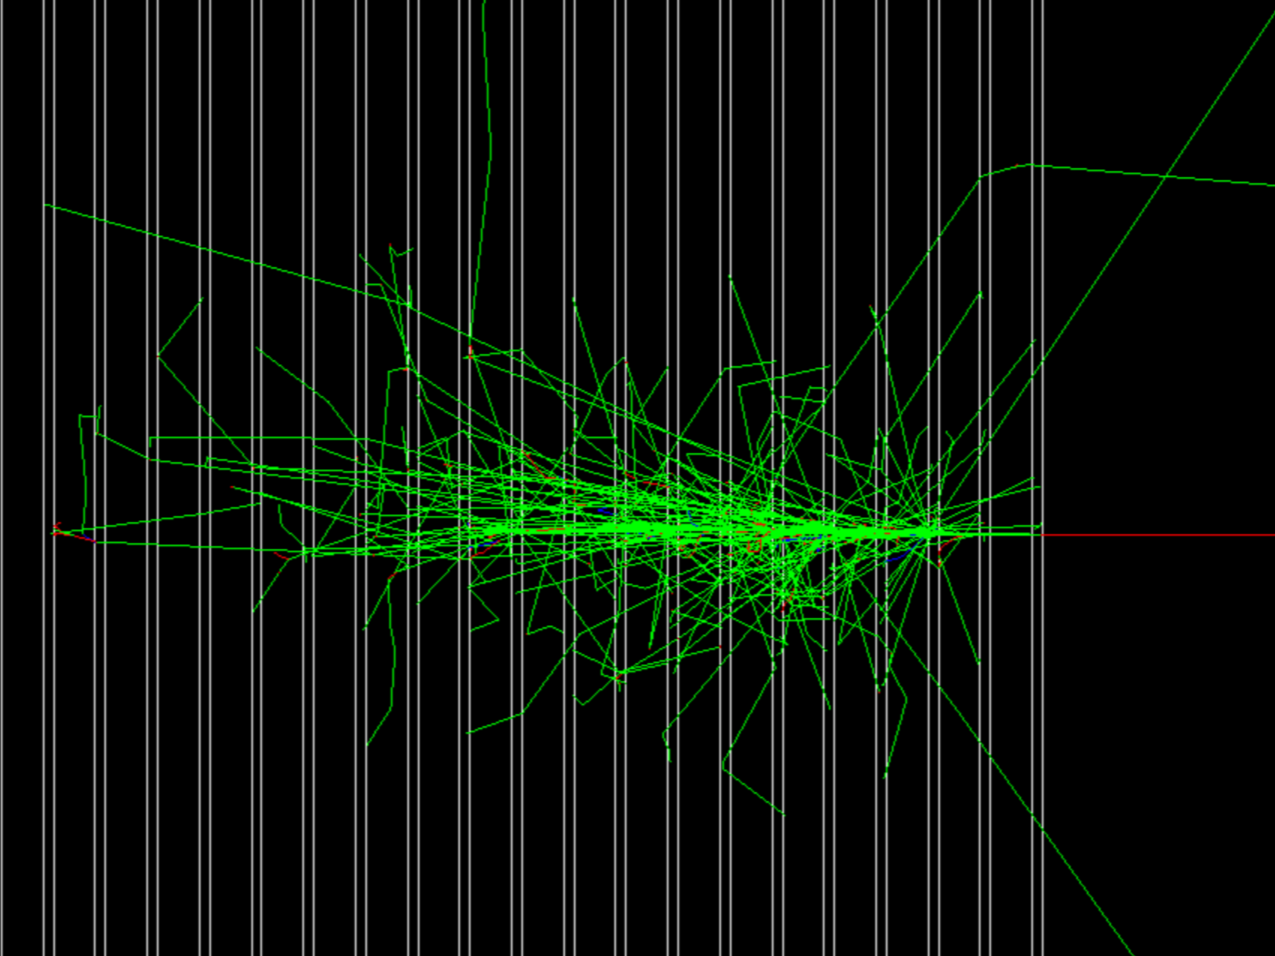
\includegraphics[width=0.75\columnwidth]{shower.png}% Here is how to import EPS art
\caption{\label{fig:epsart} Visualization of a simulated particle shower produced by a 1 GeV electron in a sampling calorimeter. Cross-sectional view is shown, with the electron incident from the right. The liquid argon and lead layers (white wire-frame) are 8 cm and 2 cm thick, respectively. Tracks are shown for particles with negative charge (red), positive charge (blue), and neutral charge (green). }
\end{figure}


\section{Data and Analysis}

- Data collected: 

    - Total energy deposited in all LAr or in all Pb layers per event.

    - Energy deposited in each LAr layer or in each Pb layer per event (position of each layer can be extracted)

- Variables

    - LAr to Pb thickness ratio: r = 0.05, 0.25, 0.5, 0.75, 0.95

    - Thickness of both layers combined: t = 10, 50, 100, 500 mm 

    - incident electron energy: Ebeam = 10, 100, 1000, 10000 MeV

- data stored in Root files

-Plot 1: Efficiency vs electron beam energy for every geometry

\onecolumngrid

\begin{figure}[H]
    \centering
    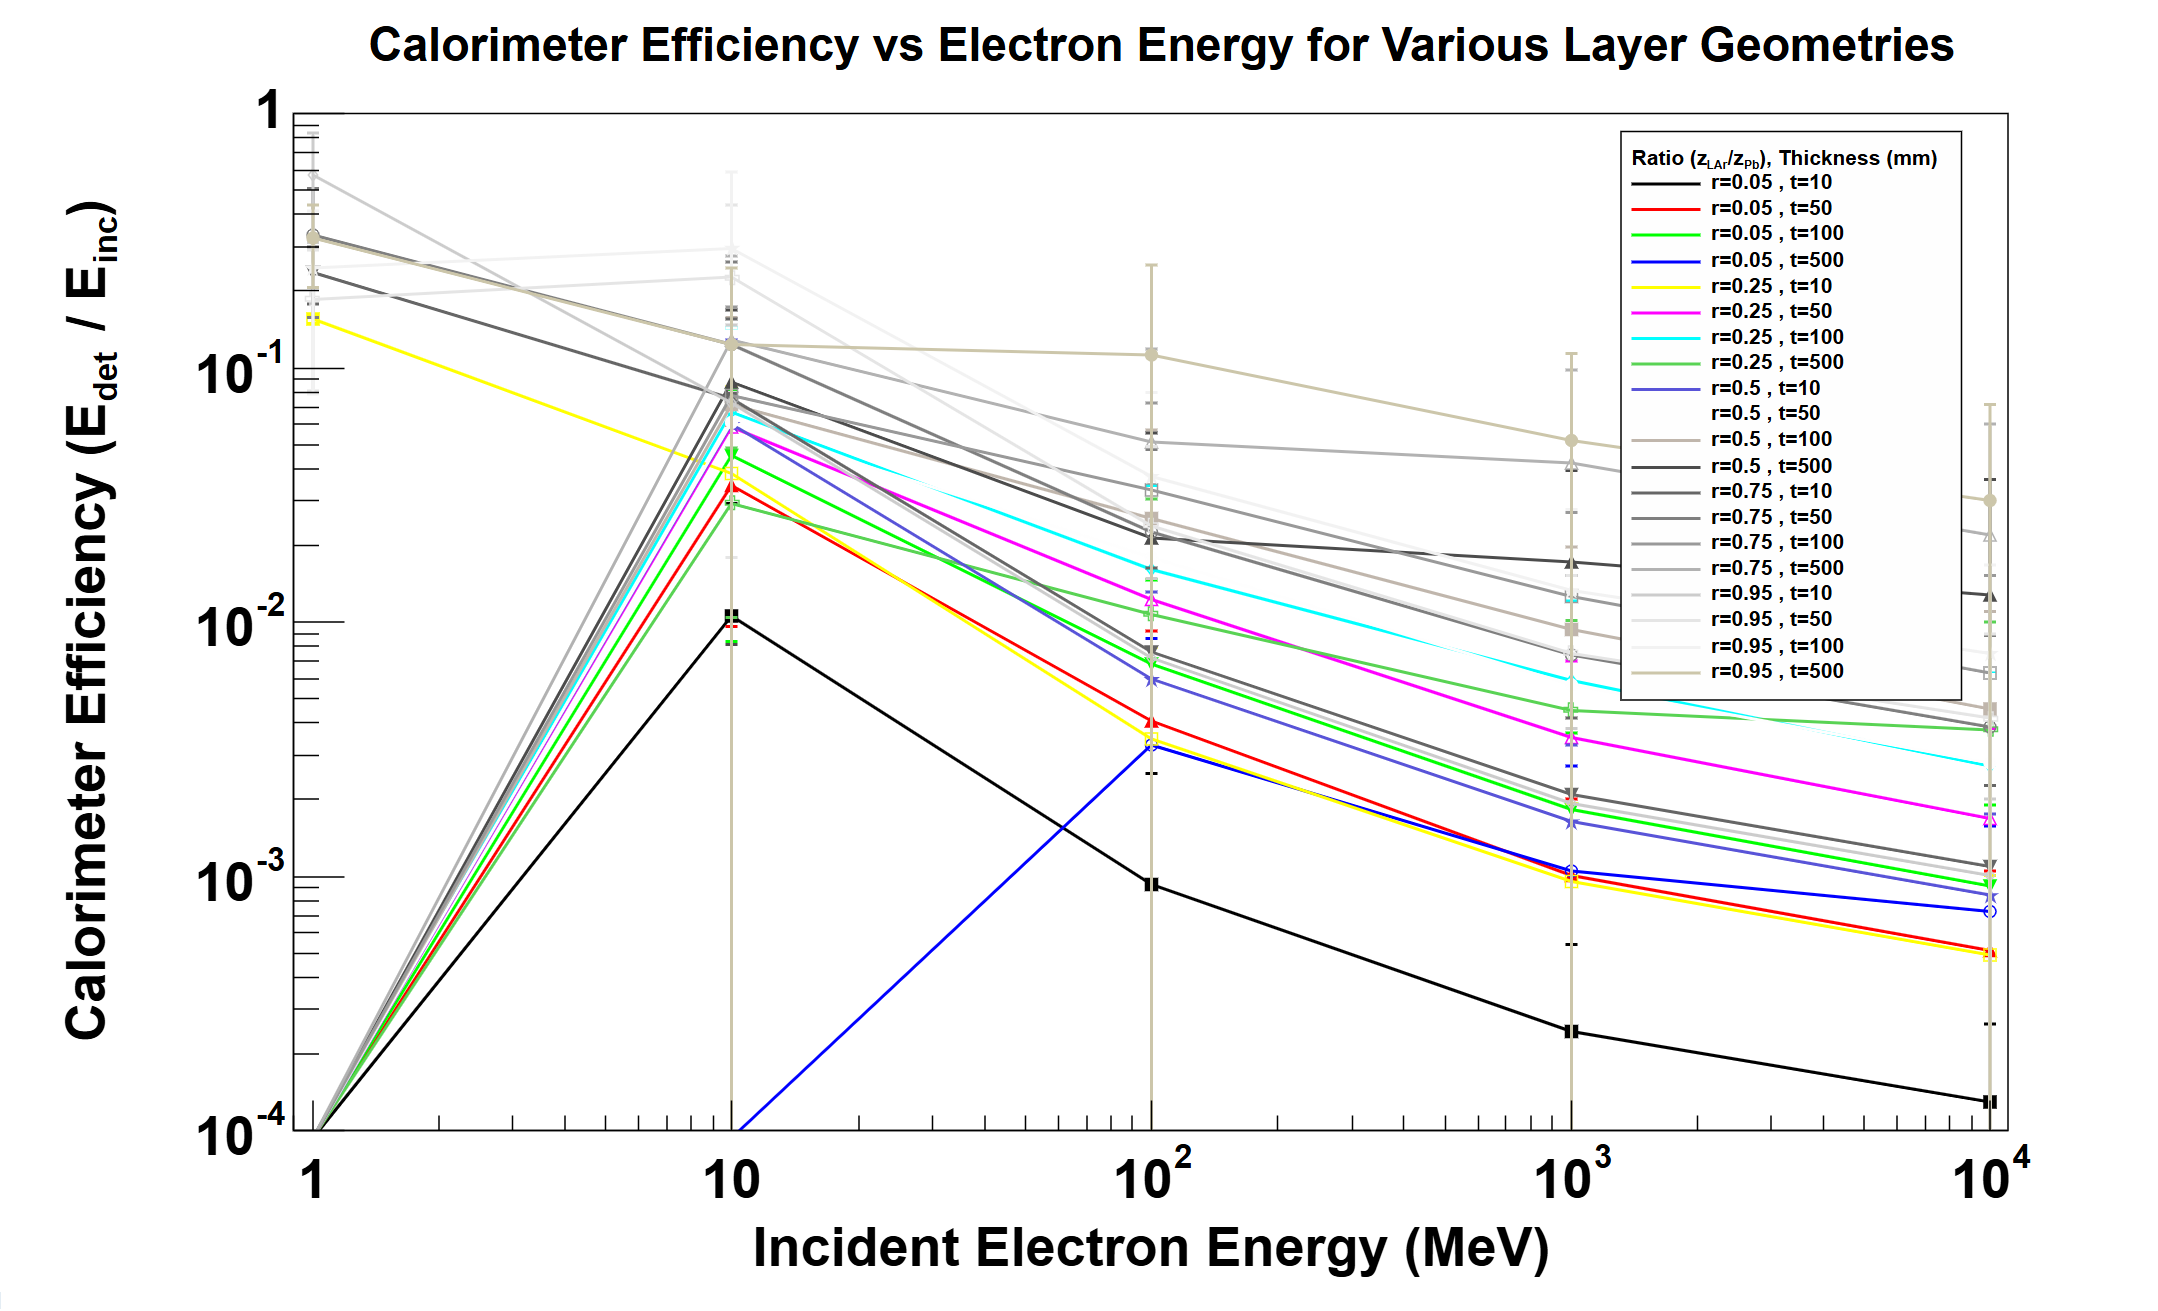
\includegraphics[width=0.75\textwidth]{efficiency2.png}% Here is how to import EPS art
    \caption{\label{fig:epsart}  }
\end{figure}
\twocolumngrid


-Plot 2: longitudinal shower profile for each electron energy (at one geometry)

Examples: ratio = 95\% Lar, layer thickness = 10mm

\begin{figure}[H]
    \centering
    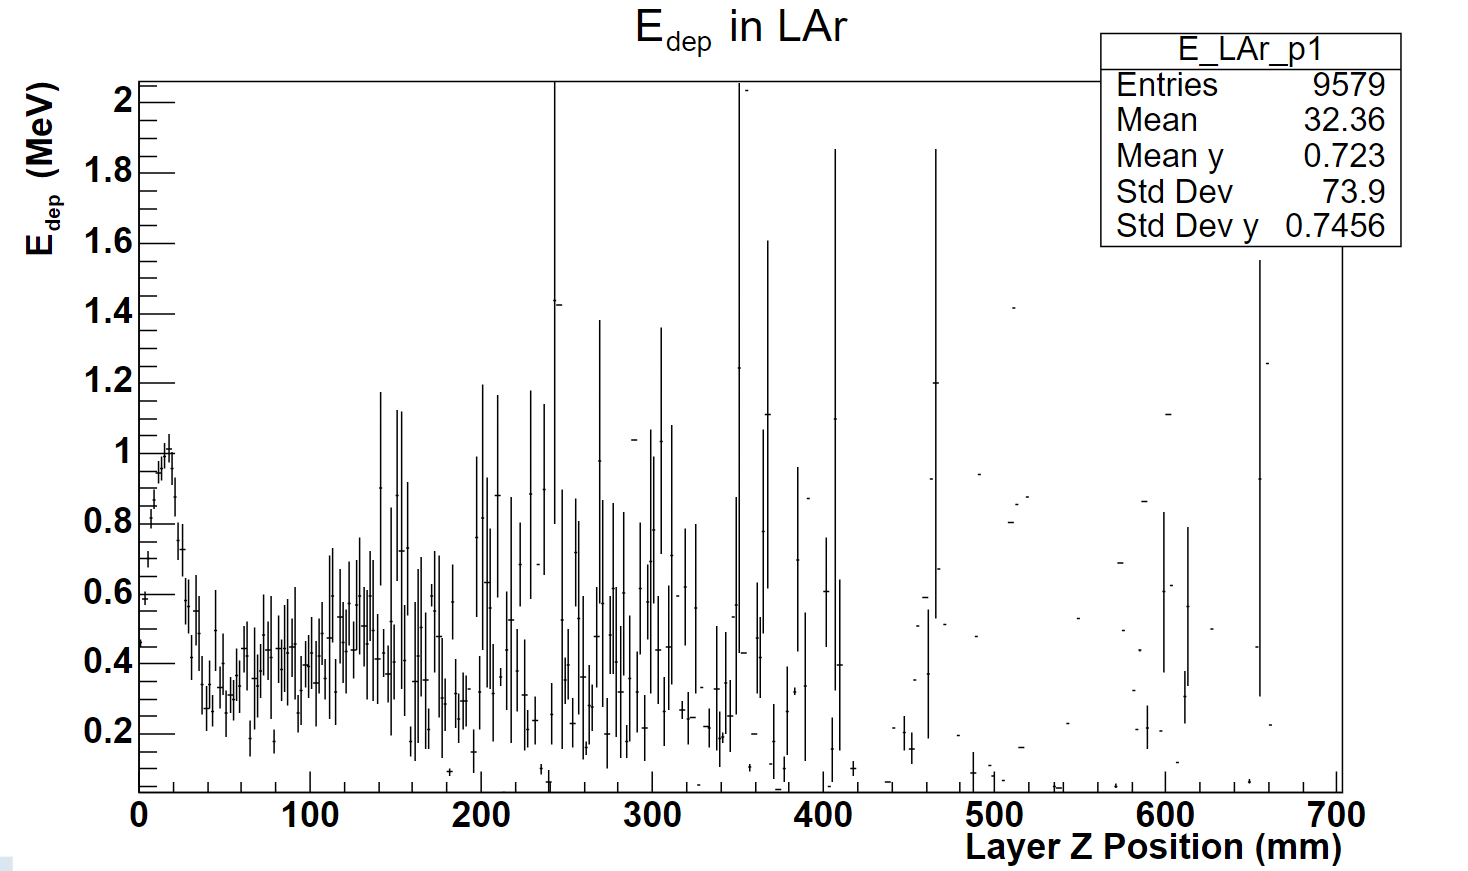
\includegraphics[width=0.9\columnwidth]{profile_0.95_10_10.png}% Here is how to import EPS art
    \caption{\label{fig:epsart} 10 MeV}
\end{figure}

\begin{figure}[H]
    \centering
    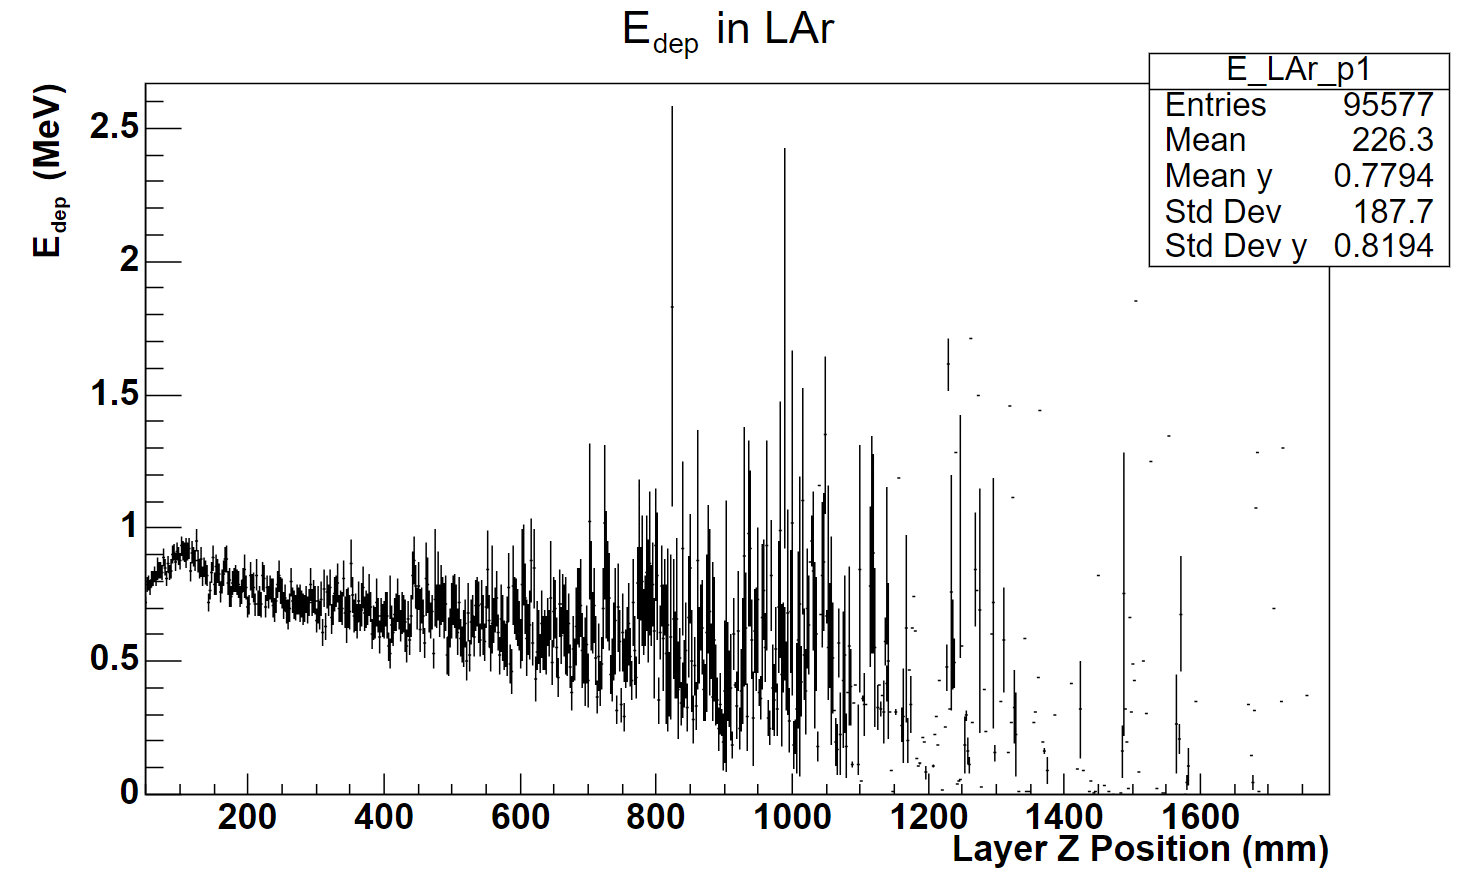
\includegraphics[width=0.9\columnwidth]{profile_0.95_10_100.png}% Here is how to import EPS art
    \caption{\label{fig:epsart} 100 MeV }
\end{figure}

\begin{figure}[H]
    \centering
    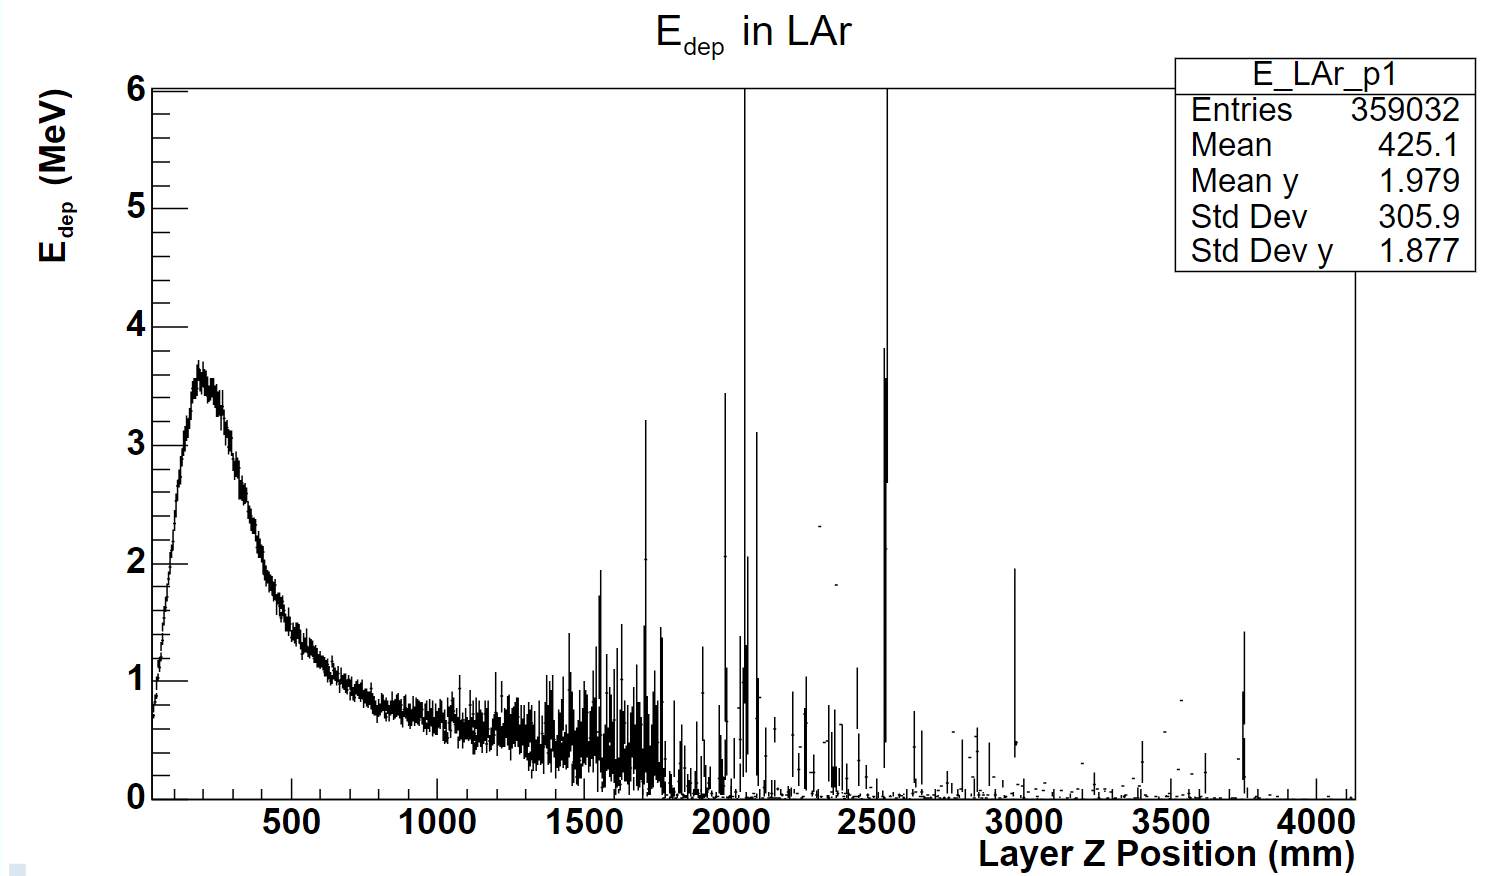
\includegraphics[width=0.9\columnwidth]{profile_0.95_10_1000.png}% Here is how to import EPS art
    \caption{\label{fig:epsart} 1 GeV }
\end{figure}

\begin{figure}[H]
    \centering
    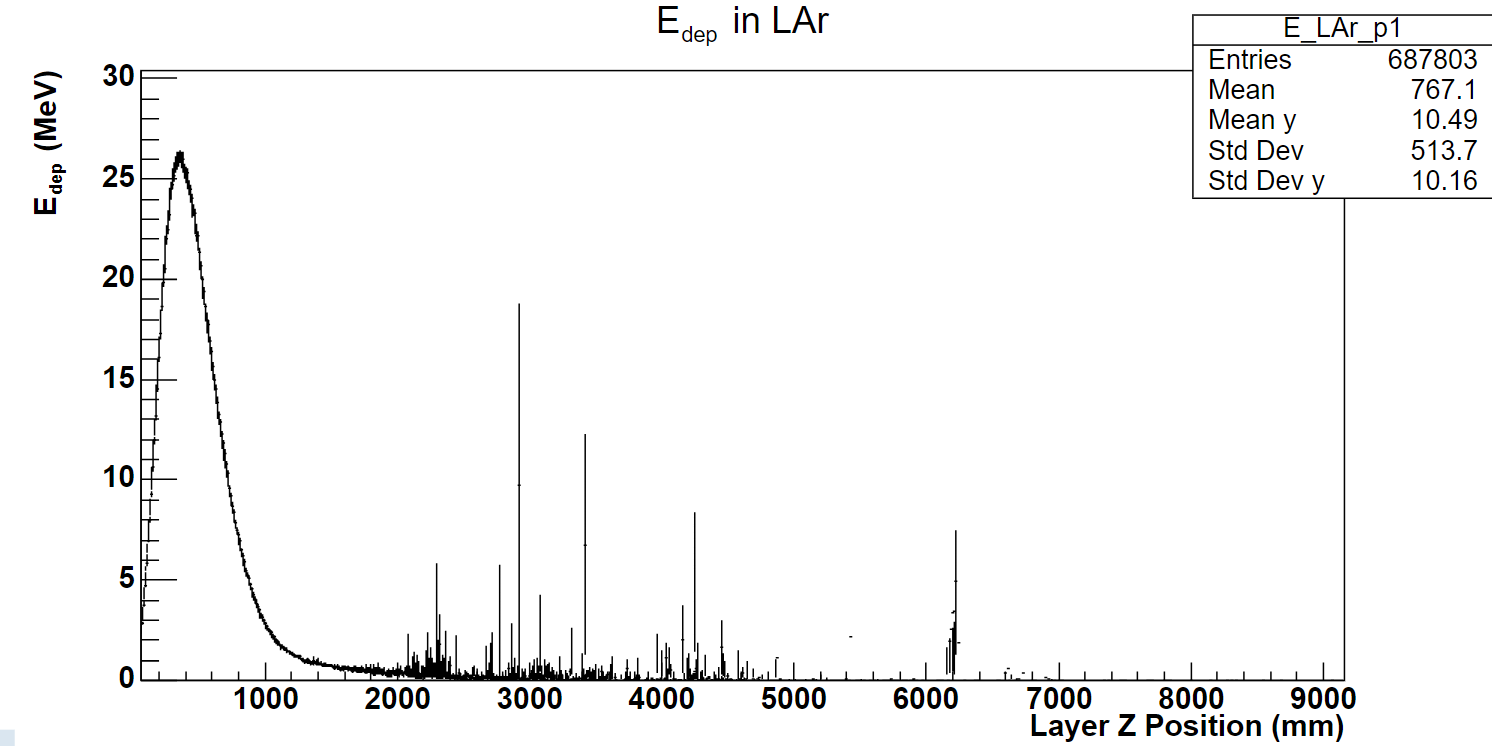
\includegraphics[width=0.9\columnwidth]{profile_0.95_10_10000.png}% Here is how to import EPS art
    \caption{\label{fig:epsart} 10GeV }
\end{figure}


-Plot 3: longitudinal profile for each geometry (at one electron energy)

Examples: longitudental energy deposition profile for electron energy of 1 GeV and layer thickness of 50mm. Varying LAr/Pb ratio

\begin{figure}[H]
    \centering
    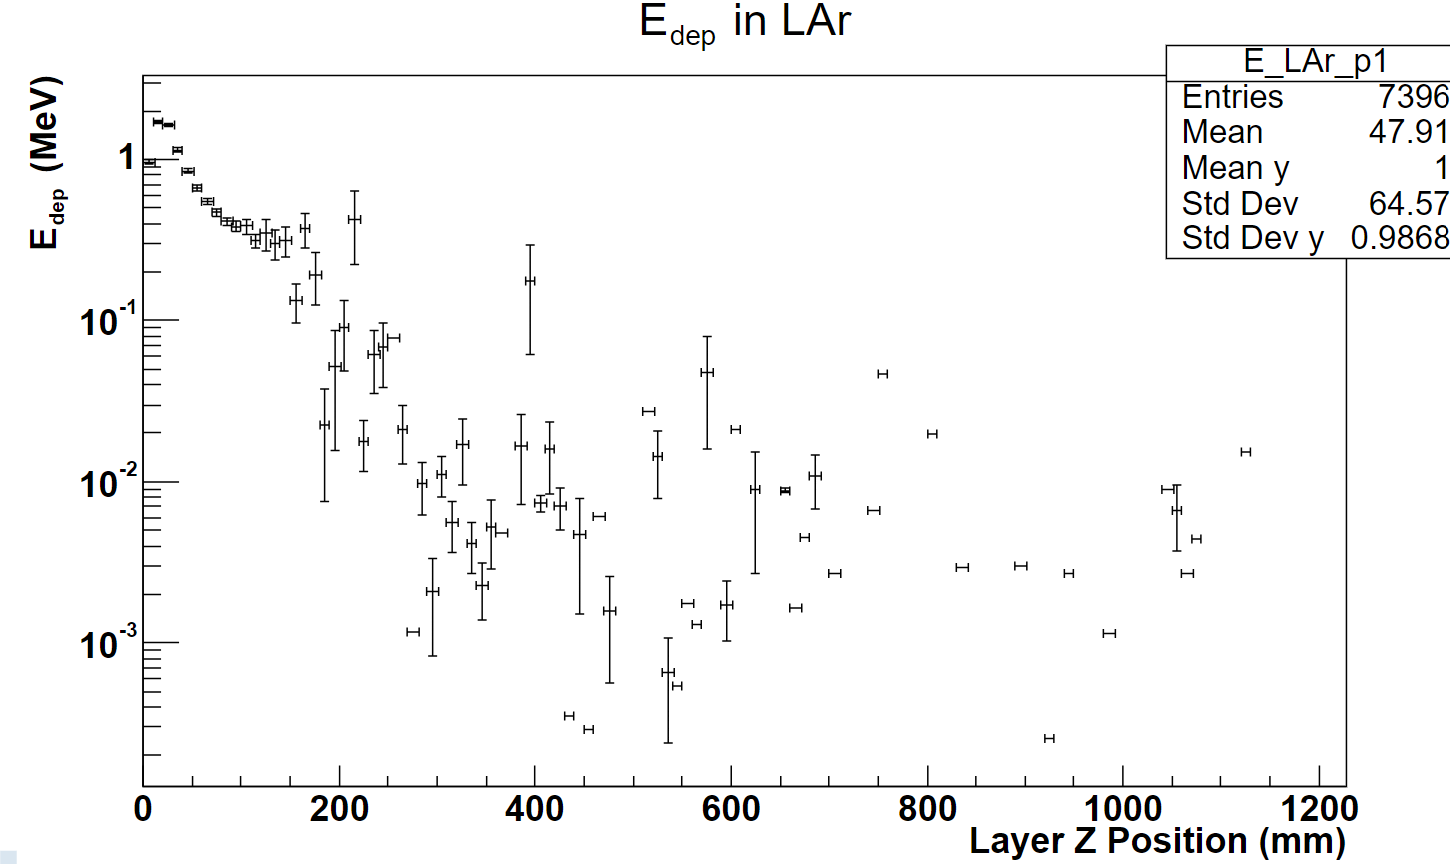
\includegraphics[width=0.9\columnwidth]{profile_0.05_50_1000.png}% Here is how to import EPS art
    \caption{\label{fig:epsart} 5\% LAr}
\end{figure}

\begin{figure}[H]
    \centering
    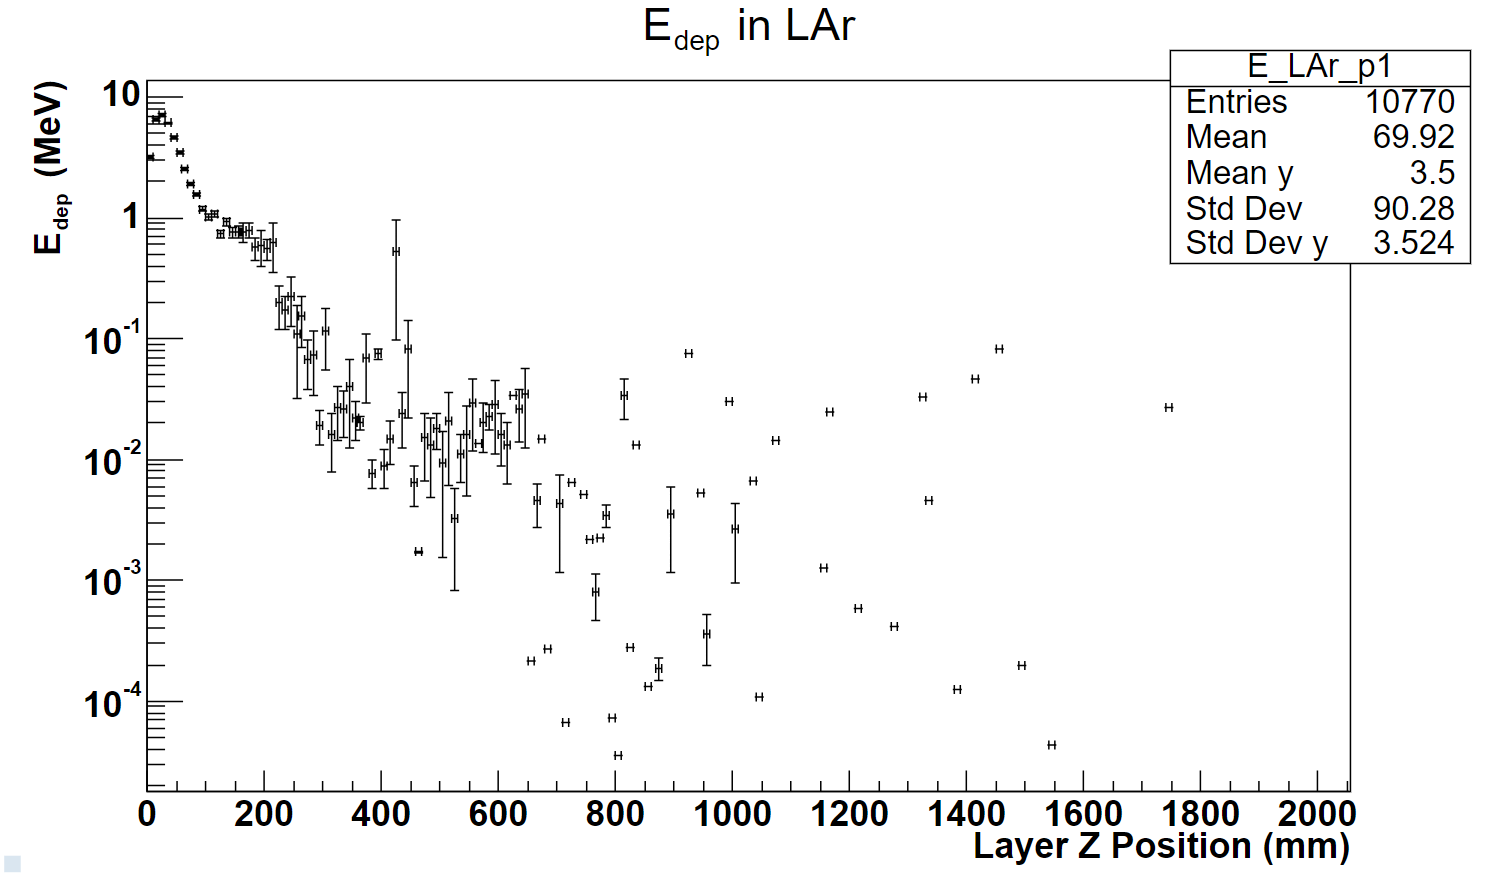
\includegraphics[width=0.9\columnwidth]{profile_0.25_50_1000.png}% Here is how to import EPS art
    \caption{\label{fig:epsart} 25\% LAr }
\end{figure}

\begin{figure}[H]
    \centering
    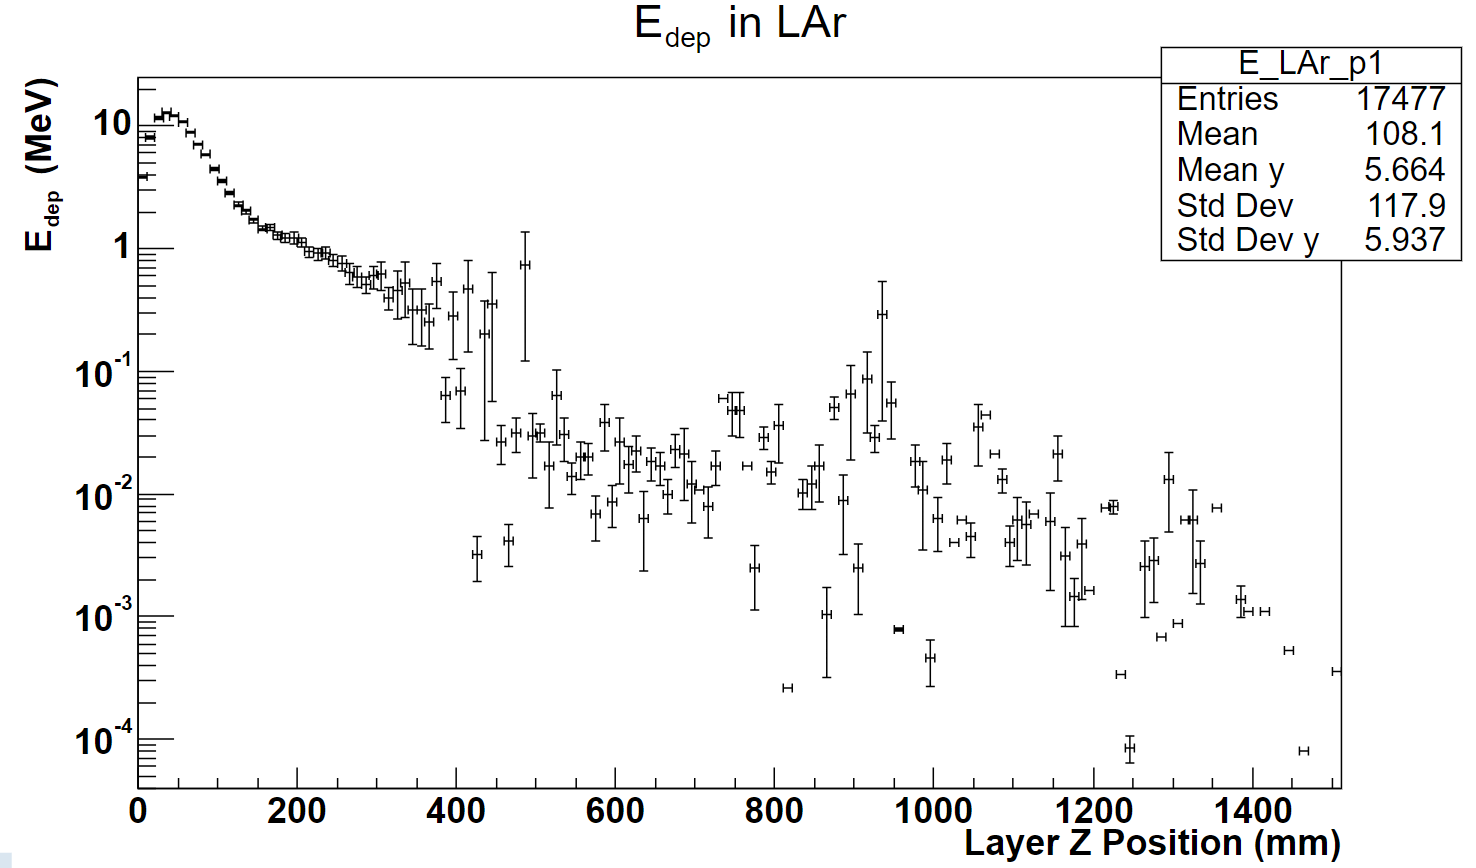
\includegraphics[width=0.9\columnwidth]{profile_0.5_50_1000.png}% Here is how to import EPS art
    \caption{\label{fig:epsart} 50\% LAr }
\end{figure}

\begin{figure}[H]
    \centering
    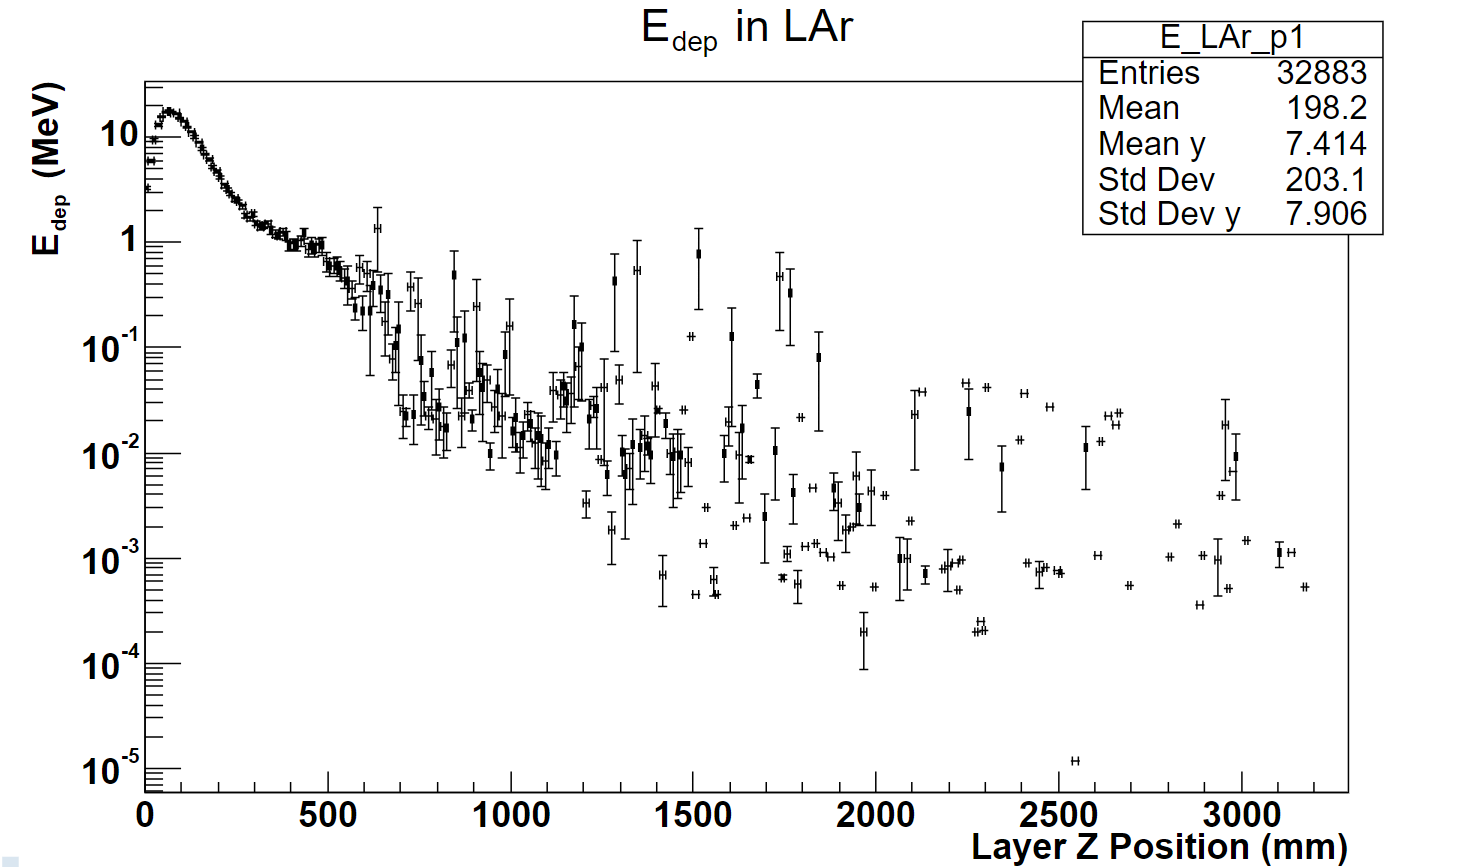
\includegraphics[width=0.9\columnwidth]{profile_0.75_50_1000.png}% Here is how to import EPS art
    \caption{\label{fig:epsart} 75\% Lar }
\end{figure}

\begin{figure}[H]
    \centering
    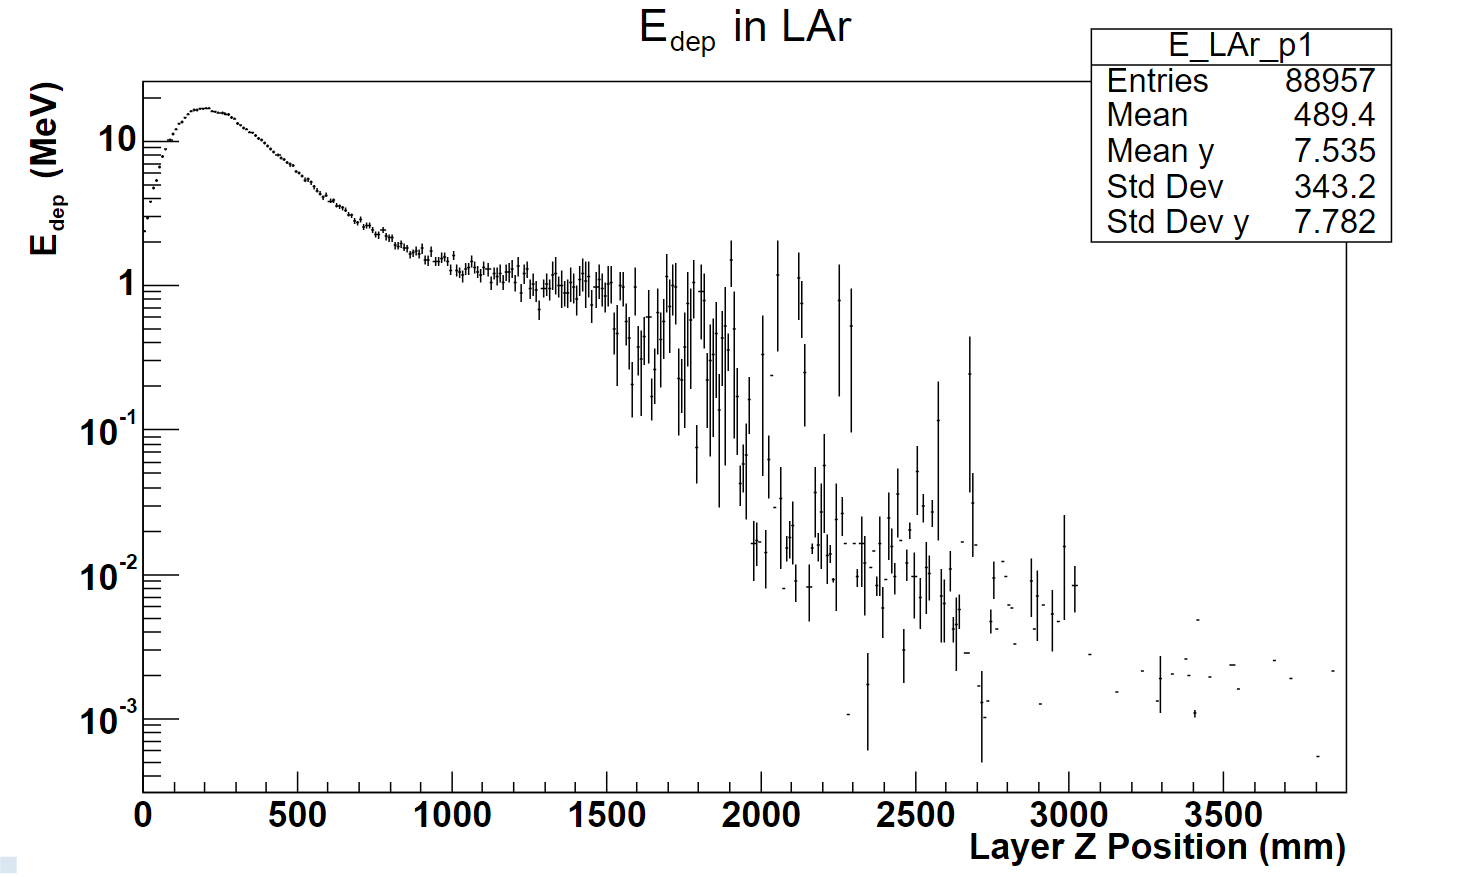
\includegraphics[width=0.9\columnwidth]{profile_0.95_50_1000.png}% Here is how to import EPS art
    \caption{\label{fig:epsart} 95\% Lar }
\end{figure}


\section{Conclusion}

- simulation physics perhaps not very accurate. How is energy deposition modeled?

- energy efficiency is very low all around -- captures 10\% of electron energy at best


\begin{acknowledgments}

[Acknowledgements]

\end{acknowledgments}


\appendix


\bibliography{main}% Produces the bibliography via BibTeX.

\end{document}
%
% ****** End of file apssamp.tex ******
